% Figure pour illustrer les fonctions à choisir pour montrer que le
% dual de C[0, 1] n'est pas séparable.
\begin{figure}[!h]
  \begin{center}
    \caption{Fonction $f$ illustrant $\|\ev_t-\ev_s\|\geq 1$}%
    \label{sepa:ill}
    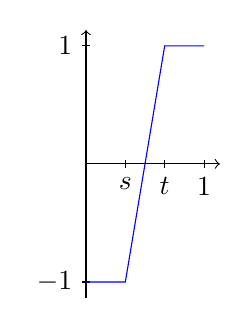
\begin{tikzpicture}[scale=0.5]
      \draw [->] (0, -3.4) -- (0, 3.4);
      \draw [->] (0, 0) -- (3.4, 0);
      \draw (1, 0.1) -- (1, -0.1) node [below] {$s$};
      \draw (2, 0.1) -- (2, -0.1) node [below] {$t$};
      \draw (3, 0.1) -- (3, -0.1) node [below] {$1$};
      \draw (0.1, 3) -- (-0.1, 3) node [left] {$1$};
      \draw (0.1, -3) -- (-0.1, -3) node [left] {$-1$};
      \draw [blue] (0, -3) -- (1 , -3) -- (2, 3) -- (3, 3);
    \end{tikzpicture}
\end{center}
\end{figure}


%%% Local Variables:
%%% mode: latex
%%% TeX-master: "../analyse3"
%%% End:
